\chapter{I sensori di presenza}
\label{chap:sensori}

Questo capitolo introduce i principi fisici alla base delle tecnologie di rilevamento considerate, analizzandone il funzionamento e le caratteristiche principali. L'analisi permette di comprendere come i diversi fenomeni fisici vengano sfruttati per rilevare la presenza di una persona e come questi si riflettano nel comportamento dei sensori.

In particolare, la Sezione~\ref{sec:pir} descrive il sensore PIR, il suo principio di funzionamento e il motivo per cui non rileva un corpo immobile. La Sezione~\ref{sec:mmwave} presenta il radar FMCW a 24 GHz, il concetto di gate di distanza e il modo in cui rileva una persona ferma. La Sezione~\ref{sec:altre} richiama brevemente le altre tecnologie di rilevamento di presenza, non considerate nel confronto sperimentale. Infine, la Sezione~\ref{sec:confronto} mette a confronto PIR e mmWave e indica in quali scenari ciascuno dei due è preferibile.


\section{Il sensore PIR}
\label{sec:pir}

\subsection{Principio fisico}
\label{subsec:pir-principio}

PIR è l'acronimo di Passive InfraRed. Il sensore non emette nulla e si limita a osservare la radiazione infrarossa che lo raggiunge. Il cuore del componente è un cristallo piroelettrico, un materiale che genera una piccola carica elettrica quando la radiazione incidente cambia. Il corpo umano, con una temperatura di circa 36 °C (309 K), emette con un picco intorno a 9,4 µm, e il sensore è filtrato con una finestra ottica di 5–14 µm proprio per privilegiare quella banda \cite{niceraPyro}.

Il comportamento del PIR dipende dalla sua capacità di rilevare le variazioni della radiazione infrarossa che raggiunge il sensore, e non la quantità di radiazione presente in un determinato istante. Costruttivamente, il sensore contiene due elementi piroelettrici disposti in configurazione differenziale, collegati in serie con polarità opposte. Da questa configurazione seguono due conseguenze fondamentali (Figura~\ref{fig:pir-detection}):

\begin{itemize}
    \item una persona che si muove investe i due elementi in tempi diversi, generando una differenza tra i segnali prodotti e quindi un rilevamento;

    \item una persona ferma illumina entrambi gli elementi con un flusso infrarosso pressoché costante. I due contributi si compensano e il segnale differenziale tende a zero, impedendo il rilevamento.
\end{itemize}

\begin{figure}[!htbp]
  \centering
  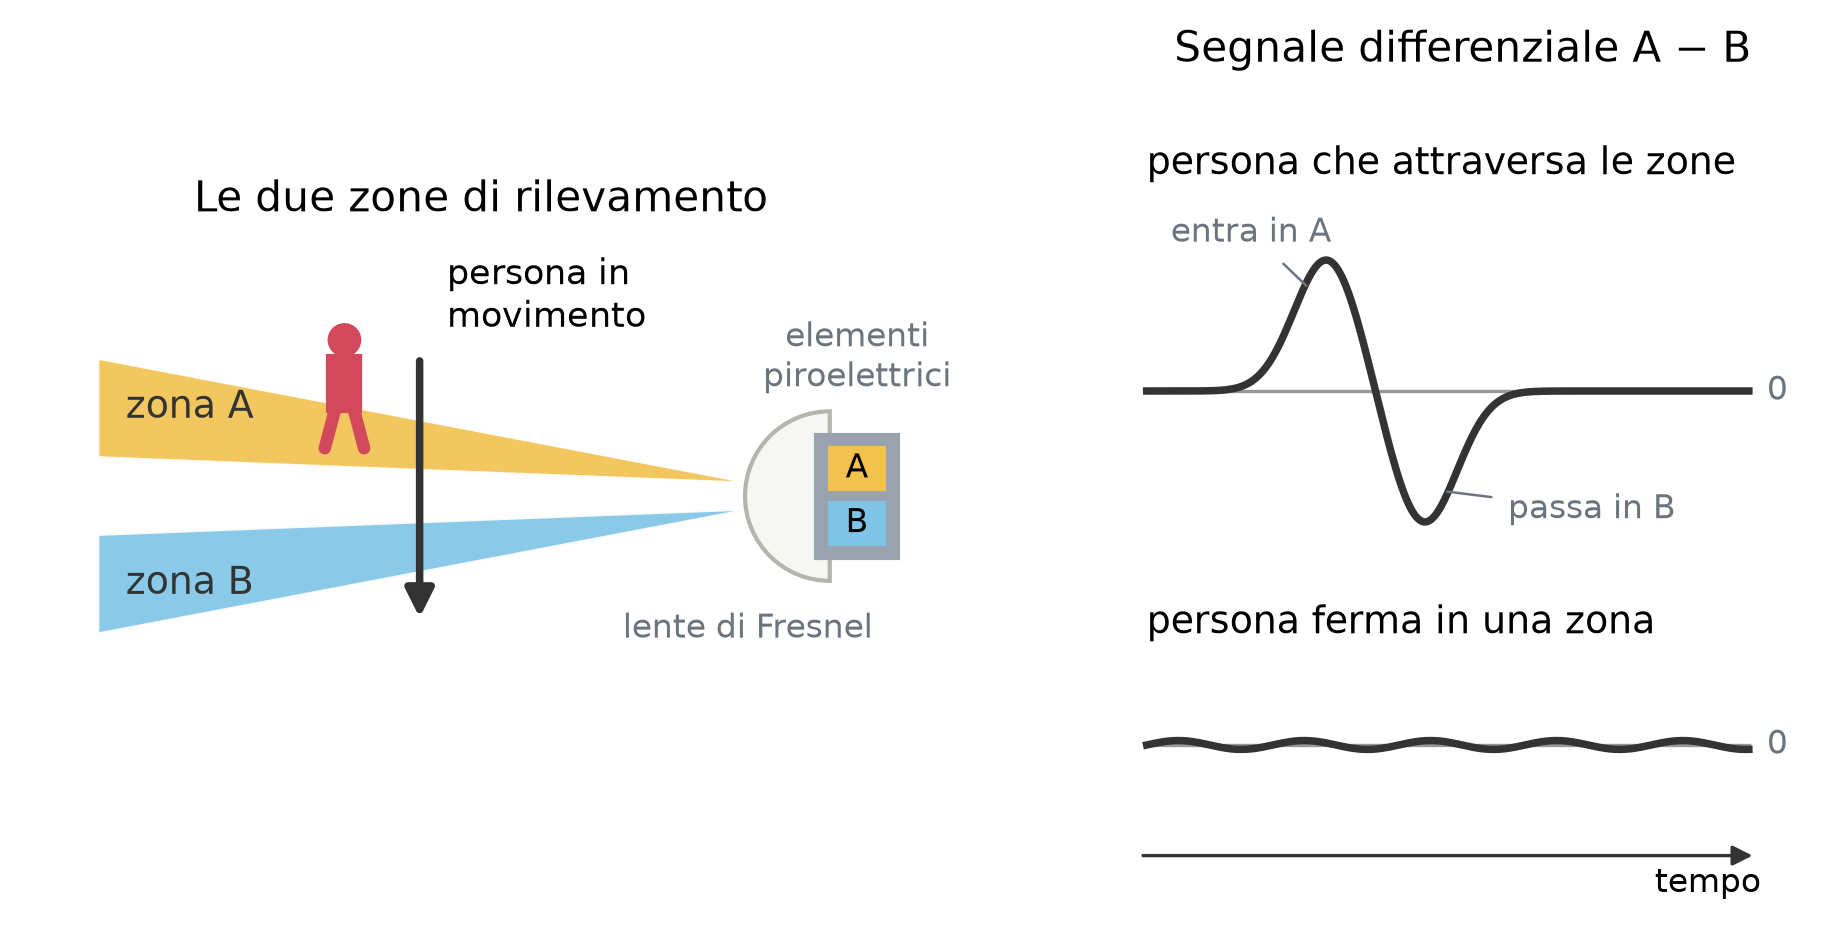
\includegraphics[width=0.8\linewidth]{Immagini/Pir_detection}
  \caption{Sensore piroelettrico a due elementi in configurazione differenziale. Una persona che attraversa le due zone le investe in tempi diversi e produce un segnale prima positivo e poi negativo; una persona ferma in una zona illumina entrambi gli elementi allo stesso modo e il segnale differenziale resta nullo.}
  \label{fig:pir-detection}
\end{figure}

Lo stesso principio spiega la buona immunità del PIR alle variazioni lente e globali della scena, come il sole che riscalda l'ambiente. Queste interessano entrambi gli elementi allo stesso modo e si cancellano nel segnale differenziale. Il rovescio della medaglia è che il segnale utile dipende dal contrasto termico fra corpo e sfondo. Con una temperatura ambiente di 20~°C il contrasto è di circa 16~°C, mentre a 30--32~°C si riduce a 4--6~°C, con segnale più debole e portata ridotta \cite{hcsr501}.

In definitiva, poiché il rilevamento richiede una variazione della radiazione infrarossa tra i due elementi, un PIR non può rilevare un corpo immobile.

\subsection{La lente di Fresnel}
\label{subsec:fresnel}

Due soli elementi coprirebbero un campo visivo strettissimo. La cupola bianca che si vede su tutti i moduli PIR è una lente di Fresnel multi-segmento. Ogni segmento focalizza sul cristallo una porzione differente della scena, e l'insieme crea decine di zone di rilevamento disposte a ventaglio e separate da zone cieche
\cite{adafruitPIR}, come mostra la Figura~\ref{fig:zone-fresnel}.

\begin{figure}[!htbp]
  \centering
  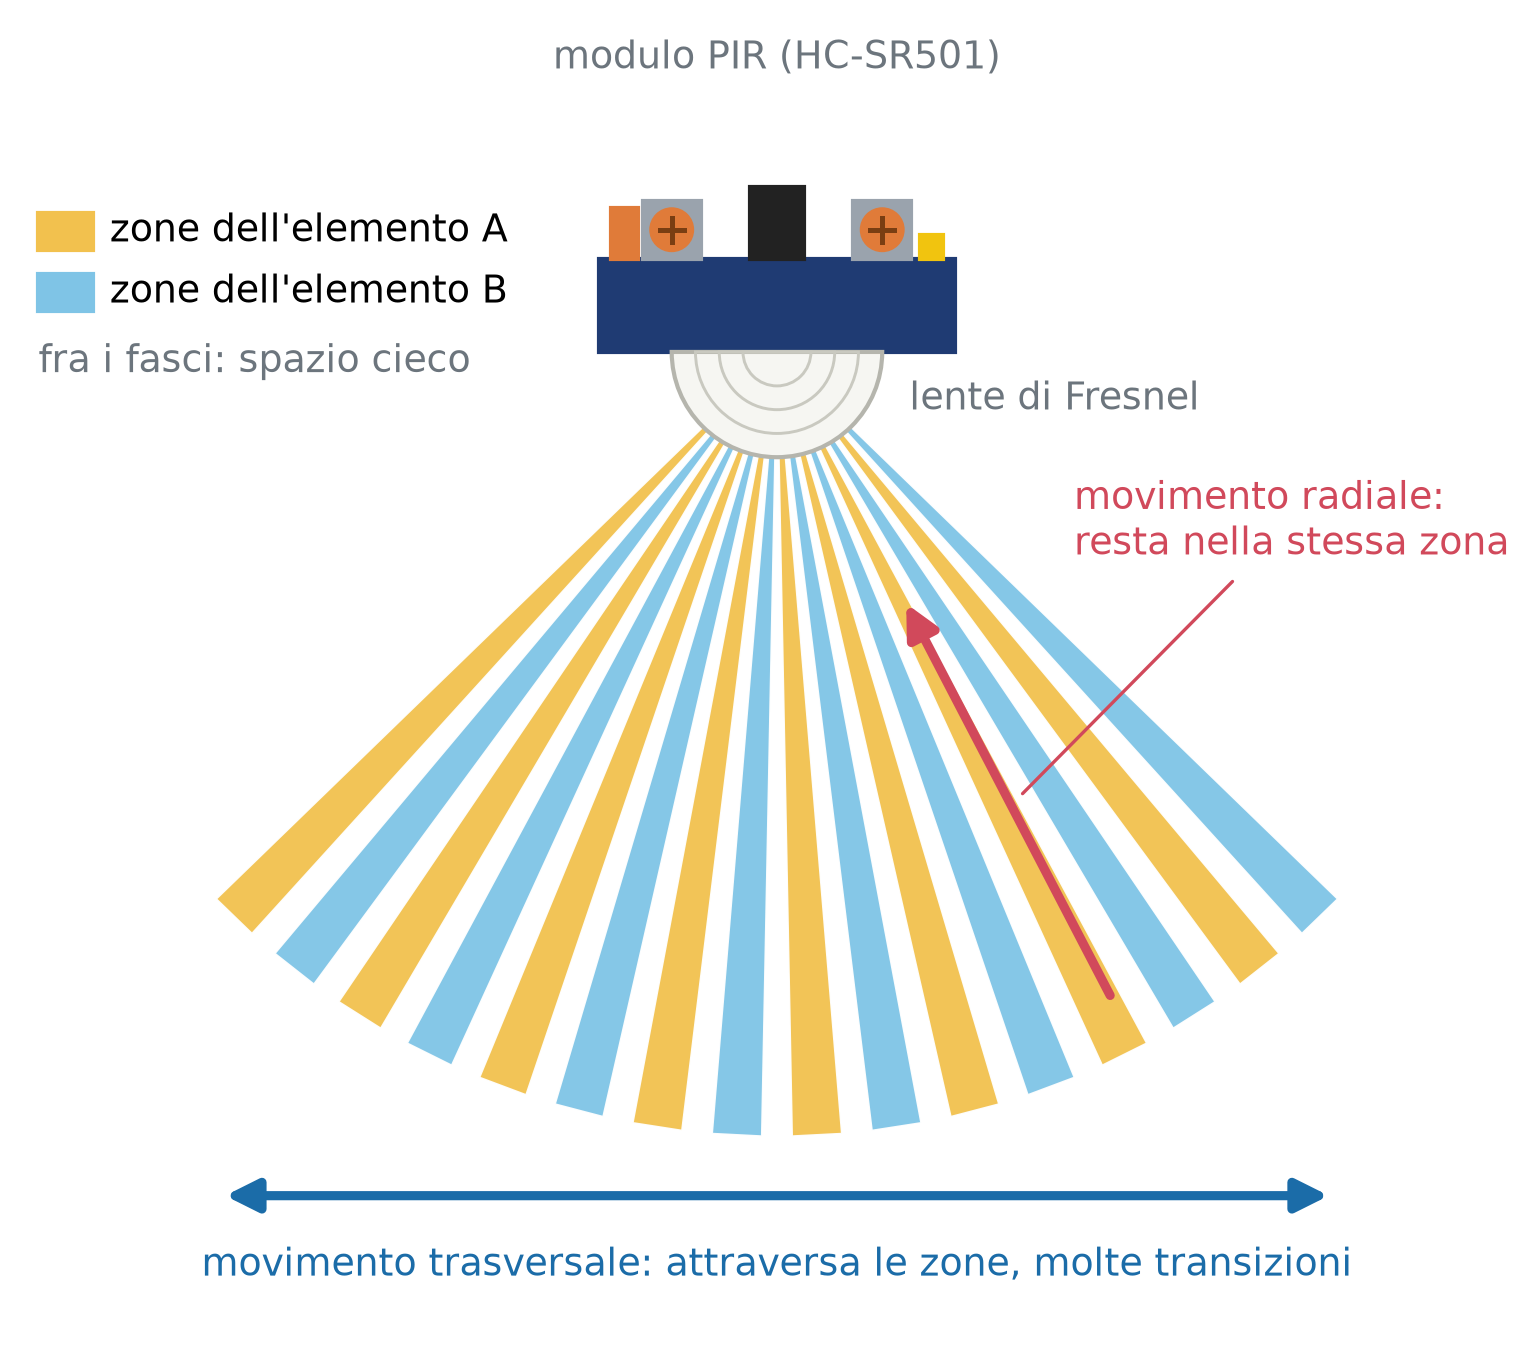
\includegraphics[width=0.6\linewidth]{Immagini/Zone_lente_fresnel}
  \caption{Zone di rilevamento create dalla lente di Fresnel, focalizzate alternativamente sui due elementi e separate da spazi ciechi. Un movimento trasversale attraversa molte zone, un movimento radiale resta nella stessa zona.}
  \label{fig:zone-fresnel}
\end{figure}

Questo dettaglio costruttivo ha due conseguenze dirette sul tipo di movimento che il sensore è in grado di rilevare:

\begin{enumerate}
    \item Il movimento trasversale, che attraversa le zone, genera molte transizioni di flusso ed è rilevato bene. Il movimento radiale, diretto verso il sensore, resta più a lungo nella stessa zona ed è rilevato male.

    \item La portata dichiarata, tipicamente 3--7~m, vale per il movimento trasversale di tutto il corpo. Un movimento sul posto non attraversa le zone e cade nel caso sfavorevole, a qualunque distanza.
\end{enumerate}

Queste due previsioni vengono messe alla prova nel Capitolo~\ref{chap:confronto}.

\subsection{I dati prodotti}
\label{subsec:pir-dati}

L'uscita di un modulo PIR è un solo bit digitale, alto quando il modulo dichiara movimento e basso altrimenti. Il passaggio dal segnale analogico del cristallo a questo bit avviene interamente a bordo del modulo, in un circuito integrato di condizionamento che amplifica il segnale, lo confronta con una soglia e tiene alta l'uscita per un tempo di ritenuta regolabile. Il microcontrollore che legge il sensore riceve quindi una decisione già presa e non ha accesso al segnale originario. I parametri di questo circuito nel modulo impiegato in questa tesi sono descritti nel dettaglio nel Capitolo~\ref{chap:moduli}.

Fa eccezione la modalità di trigger, selezionabile con un ponticello, perché determina il significato stesso del bit in uscita. Le modalità previste sono due (Figura~\ref{fig:pir-lh}) \cite{hcsr501}:

\begin{itemize}
    \item \textbf{Modalità L} (\textit{single trigger}). Il primo movimento alza l'uscita per il tempo di ritenuta e i movimenti successivi, finché l'uscita è alta, vengono ignorati. Allo scadere della ritenuta l'uscita torna bassa anche se la persona si sta ancora muovendo, e serve un nuovo trigger per rialzarla. Il bit si comporta come un monostabile a durata fissa e, di fatto, conta eventi.

    \item \textbf{Modalità H} (\textit{repeat trigger}). Ogni movimento rilevato durante la ritenuta la fa ripartire da zero. Finché il movimento continua l'uscita resta alta, e torna bassa solo quando il movimento cessa per un tempo pari alla ritenuta. In questa modalità la durata del bit alto segue la durata del movimento e il sensore si avvicina di più a un rilevatore di presenza.
\end{itemize}

\begin{figure}[!htbp]
  \centering
  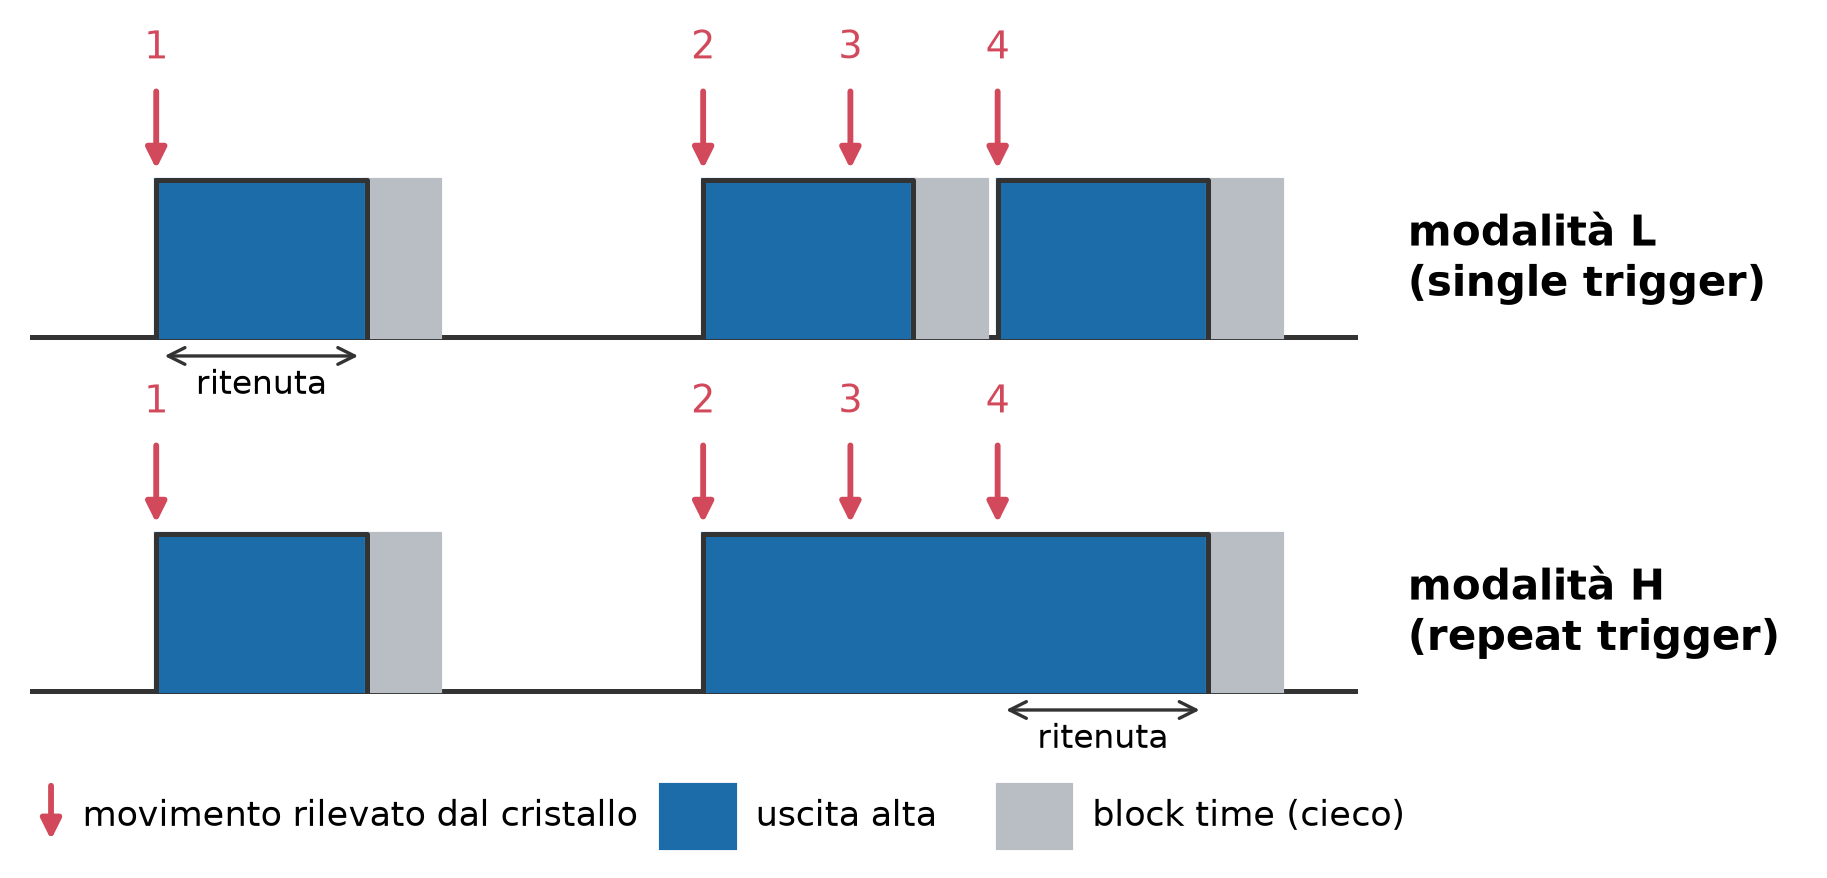
\includegraphics[width=0.9\linewidth]{Immagini/Pir_L_H}
  \caption{Uscita del PIR nelle due modalità di trigger a parità di movimenti. In L ogni
  impulso dura quanto la ritenuta e i movimenti al suo interno sono ignorati; in H ogni
  movimento riarma la ritenuta e l'uscita resta alta finché il movimento continua.}
  \label{fig:pir-lh}
\end{figure}

\FloatBarrier
\subsection{Chi lo usa e perché domina}
\label{subsec:pir-usi}

Il PIR è il sensore di presenza più diffuso al mondo e da decenni equipaggia luci automatiche, antifurti, videocitofoni e termostati. La sua diffusione si spiega con diversi fattori:

\begin{itemize}
    \item \textbf{Consumo.} La corrente di riposo è inferiore a 50~$\mu$A, compatibile con anni di funzionamento a batteria \cite{hcsr501}.

    \item \textbf{Costo.} Un modulo completo di lente e circuito di condizionamento costa pochi euro.

    \item \textbf{Semplicità.} Il modulo fornisce direttamente il bit di presenza e non richiede alcuna elaborazione a valle.

    \item \textbf{Natura passiva.} Il sensore non emette alcuna radiazione, e questo semplifica sia le certificazioni sia la conformità in materia di privacy.
\end{itemize}


\section{Il radar mmWave a 24 GHz}
\label{sec:mmwave}

\subsection{Principio di funzionamento}
\label{subsec:fmcw}

I radar di presenza di fascia consumer sono radar FMCW (\textit{Frequency Modulated Continuous Wave}) che operano nella banda ISM intorno a 24~GHz, un'allocazione libera da licenza larga 250~MHz (24,00--24,25~GHz) e disponibile in Europa e negli Stati Uniti \cite{ituRR}.

Il nome con cui vengono commercializzati, radar mmWave, è in realtà improprio. La banda delle onde millimetriche (EHF) è definita fra 30 e 300~GHz, dove la lunghezza d'onda è compresa fra 10 e 1~mm \cite{ituRR}. A 24~GHz la lunghezza d'onda vale circa 12,4~mm, quindi questi moduli lavorano ancora nella banda SHF delle onde centimetriche. La denominazione deriva dal fatto che la stessa famiglia di sensori esiste anche a 60 e 77~GHz, che sono effettivamente millimetriche, ed è ormai quella adottata dai produttori. Nella tesi si mantiene per coerenza con le fonti citate.

Il principio di funzionamento si può descrivere in quattro passi \cite{tiFmcw}:

\begin{enumerate}
    \item Il trasmettitore emette un segnale continuo la cui frequenza sale in modo lineare nel tempo, per esempio da 24,00 a 24,25~GHz in qualche millisecondo. Questa rampa si chiama \textit{chirp} e si ripete in continuazione.

    \item Il segnale colpisce un oggetto e torna al ricevitore dopo un tempo di volo pari al doppio della distanza diviso la velocità della luce. Per un oggetto a 3~m il ritardo è di circa 20~ns.

    \item In quei 20~ns il trasmettitore ha continuato a salire di frequenza, quindi, nell'istante in cui l'eco arriva, il segnale trasmesso ha una frequenza leggermente più alta. Il ricevitore mescola i due segnali e ne ottiene la differenza, detta frequenza di battimento (Figura~\ref{fig:fmcw}). Poiché la rampa è lineare, questa differenza è proporzionale al ritardo, e dunque alla distanza dell'oggetto.

    \item Se nella scena ci sono più oggetti a distanze diverse, l'eco complessiva contiene una frequenza di battimento per ciascuno. Una trasformata di Fourier del segnale ricevuto le separa e restituisce, per ogni distanza, quanta energia è stata riflessa da lì.
\end{enumerate}

\begin{figure}[!htbp]
  \centering
  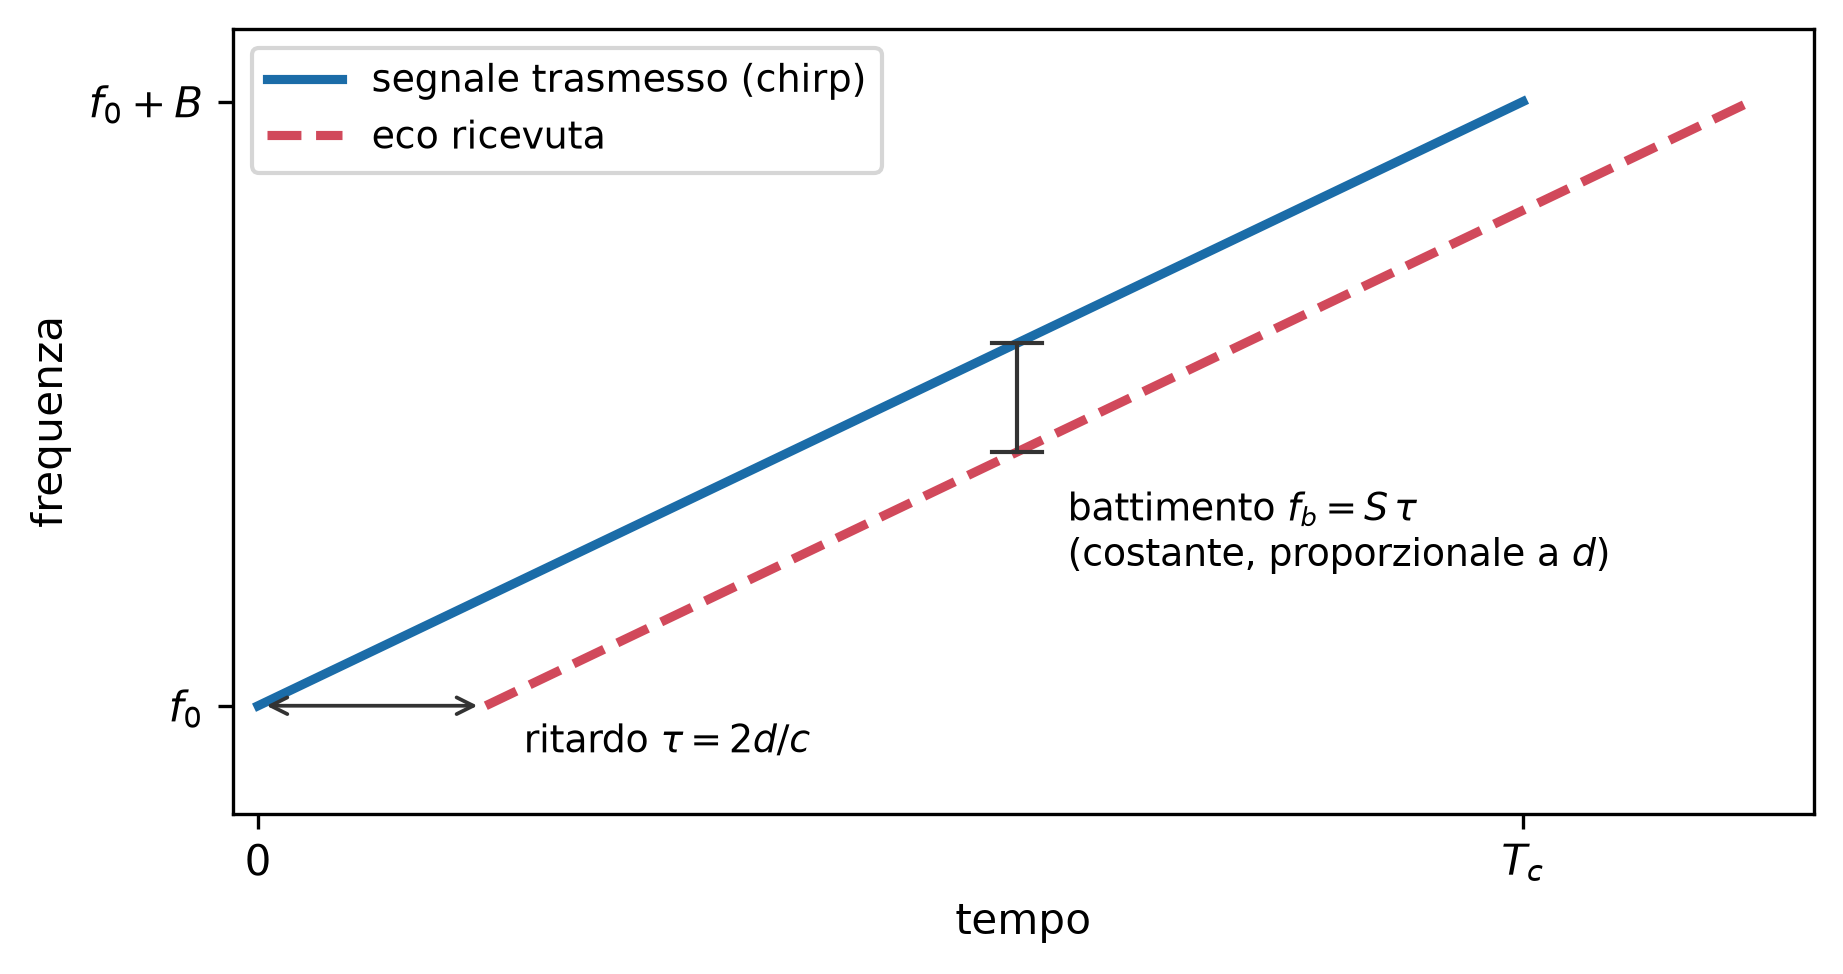
\includegraphics[width=0.75\linewidth]{Immagini/Rilevamento_segnale_radar}
  \caption{Principio FMCW. La frequenza trasmessa cresce linearmente nel tempo, l'eco torna
  con un ritardo proporzionale alla distanza e la differenza di frequenza fra i due
  segnali, costante durante il chirp, misura quel ritardo.}
  \label{fig:fmcw}
\end{figure}

Il risultato di ogni chirp è quindi un profilo che associa a ciascuna distanza un'intensità di eco. La separazione minima fra due oggetti distinguibili dipende dalla larghezza di banda della rampa e, con i 250~MHz disponibili a 24~GHz, è di circa 60~cm \cite{tiFmcw}. È per questo che i moduli di questa classe lavorano con celle di distanza di 70--75~cm.

I moduli consumer non espongono il profilo grezzo, ma una sua versione già elaborata. L'asse delle distanze è suddiviso in un numero fisso di intervalli contigui, detti gate, e per ciascun gate il modulo riporta a ogni frame un valore di energia riflessa, insieme alla decisione di presenza e alla distanza del bersaglio ricavate da quei valori. Il numero di gate, la scala dell'energia e i canali disponibili variano da modulo a modulo e sono descritti nel Capitolo~\ref{chap:moduli} per i due esemplari in esame.

\FloatBarrier
\subsection{Come si rileva un corpo immobile}
\label{subsec:corpo-immobile}

Un radar FMCW puro misura la distanza e non il movimento, quindi un corpo fermo produce comunque un'eco. In pratica, i moduli commerciali separano due contributi:

\begin{itemize}
    \item la componente \textit{moving}, associata a variazioni rapide della fase dell'eco, cioè allo spostamento del bersaglio;

    \item la componente \textit{stationary} (o \textit{motionless}), associata a un'eco stabile in distanza ma con fluttuazioni residue.
\end{itemize}

Una persona ferma non è mai realmente immobile, perché il torace si muove di alcuni millimetri a ogni atto respiratorio e, a 24~GHz, anche uno spostamento millimetrico produce una variazione di fase misurabile. È questa la ragione fisica per cui il radar può rilevare una persona immobile, a differenza del PIR. Lo stesso segnale, analizzato nel tempo, permette anche di stimare la frequenza respiratoria, come mostrato nel Capitolo~\ref{chap:vitalita}.

\subsection{Applicazioni e diffusione}
\label{subsec:mmwave-usi}

I radar mmWave di fascia consumer si sono diffusi negli ultimi anni in diversi ambiti, per esempio nell'illuminazione automatica di uffici e abitazioni, nell'automazione degli edifici per stimare l'occupazione degli ambienti, nel monitoraggio del sonno e nei sistemi di rilevamento delle cadute per l'assistenza agli anziani \cite{mmwaveOccupancy}. In ambito di ricerca gli stessi radar sono impiegati per il monitoraggio senza contatto dei parametri vitali, in particolare della frequenza respiratoria e cardiaca \cite{upm2024vitals,uts2024vitals,mdpi2024mmwaverm}. La loro diffusione si spiega con diversi fattori:

\begin{itemize}
    \item \textbf{Rilevamento del corpo fermo.} Il modulo conferma la presenza di una persona anche quando è immobile, grazie alla sensibilità ai micro-movimenti descritta nella Sezione~\ref{subsec:corpo-immobile}.

    \item \textbf{Informazione graduata.} Oltre alla presenza il modulo riporta la distanza del bersaglio e un'energia riflessa per ogni gate, che permettono di sapere non solo se c'è qualcuno ma dove si trova e quanto si muove.

    \item \textbf{Insensibilità alle condizioni ambientali.} La misura non dipende dalla temperatura né dall'illuminazione, e le onde a 24 GHz attraversano vari materiali, per cui il modulo può essere nascosto dietro una copertura.

    \item \textbf{Privacy.} Il radar non produce immagini e non permette di riconoscere una persona, e per questo è accettato in ambienti sensibili come scuole o camere da letto. I dati grezzi per gate permettono però di ricavare anche grandezze sullo stato fisico, come il respiro. In questa tesi sono esportati integralmente per l'analisi, mentre in un'installazione reale andrebbero trattati con le cautele del GDPR indicate dal progetto per gli ambienti scolastici~\cite{callisto2026dipme}.

    \item \textbf{Costo.} I moduli integrati, completi di antenne ed elaborazione a bordo, costano nell'ordine della decina di euro e forniscono i dati già elaborati su una porta seriale.
\end{itemize}

Il lato negativo è il consumo. Un radar è un sensore attivo, che deve alimentare un trasmettitore e un'elaborazione continua del segnale, e la sua corrente di alimentazione è dell'ordine delle decine di milliampere. Questo ne condiziona l'impiego nei dispositivi a batteria.


\FloatBarrier
\section{Altre tecnologie di rilevamento di presenza}
\label{sec:altre}

Oltre al PIR e al radar mmWave esistono altre tecnologie in grado di rilevare la presenza di una persona. Di seguito se ne descrivono alcune, nessuna delle quali è stata presa in considerazione nel confronto sperimentale di questa tesi.

\textbf{UWB (Ultra-WideBand).} È una tecnologia radio che trasmette impulsi molto brevi su una banda larga alcuni gigahertz, tipicamente fra 3 e 10 GHz. La brevità degli impulsi dà un'ottima risoluzione temporale, e quindi spaziale, che la rende adatta soprattutto alla misura di distanza fra dispositivi. Usata come radar è in grado di rilevare corpi fermi e di attraversare i materiali, con consumi contenuti \cite{rfwireless}. I moduli disponibili forniscono però dati grezzi che richiedono un'elaborazione dedicata, e il loro impiego principale resta la localizzazione, non il rilevamento di presenza in un volume.

\textbf{Ultrasuoni.} Un trasduttore emette un impulso acustico e misura il tempo di ritorno dell'eco. Sono economici e precisi sulla distanza, ma il segnale è assorbito dai tessuti e dipende fortemente dalla geometria della scena, per cui la presenza umana viene rilevata in modo poco affidabile.

\textbf{CO$_2$.} La concentrazione di anidride carbonica cresce con il numero di persone in un ambiente ed è un buon indicatore della sua occupazione complessiva. Il gas però si diffonde lentamente, con tempi di risposta dell'ordine dei minuti, e la misura non dà alcuna informazione su dove si trovino le persone.

\textbf{Visione.} Telecamere e termocamere sono la soluzione più ricca di informazione, perché permettono di contare, localizzare e riconoscere le persone. Richiedono però un'elaborazione pesante, costano di più e producono immagini, e questo pone vincoli di privacy che negli ambienti scolastici e domestici ne limitano fortemente l'impiego.

 
 \section{PIR e mmWave a confronto}
\label{sec:confronto}

 Le caratteristiche elencate nelle Sezioni~\ref{subsec:pir-usi} e~\ref{subsec:mmwave-usi} mostrano che PIR e radar mmWave non sono alternative equivalenti, ma rispondono a esigenze diverse.

Il PIR è la scelta giusta quando l'obbiettivo è rilevare il passaggio o l'attività di una persona e il dispositivo deve funzionare a batteria per lungo tempo. Il suo limite è strutturale e non dipende dal modello o dalla configurazione. Per il principio descritto nella Sezione~\ref{subsec:pir-principio} non rileva un corpo immobile, e per la geometria della lente descritta nella Sezione~\ref{subsec:fresnel} rileva male anche chi si muove senza spostarsi. È quindi inadatto ogni volta che la persona da rilevare può stare ferma.

Il radar mmWave è preferibile quando serve confermare la presenza di una persona immobile, oppure sapere dove si trova e quanto si muove. Il suo limite è il consumo, che ne condiziona l'uso continuo a batteria. Queste capacità e questo limite sono verificati sperimentalmente nel Capitolo~\ref{chap:confronto} e analizzati nel Capitolo~\ref{chap:consumi}.